\begin{minipage}{.45\textwidth}
	\begin{figure}[H]
		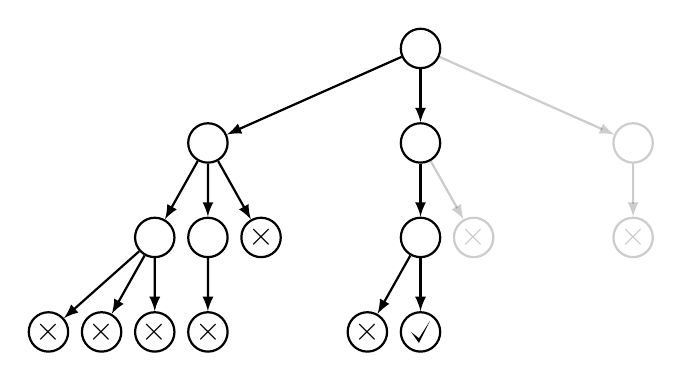
\begin{tikzpicture}[scale=.75, x=9mm, y=8mm]
			\def\checkmark{\tikz\fill[x=4mm, y=4mm](0, .35) -- (.25, 0) -- (.6, .7) -- (.25, .15) -- cycle;} 
			\tikzstyle{node}=[draw, thick, circle, inner sep=0pt, minimum width=5mm]
			\large
			\node[node] (a) at (0, 6) {};
			\node[node] (b1) at (-4, 4) {};
			\node[node] (b2) at (0, 4) {};
			\node[node, opacity=.2] (b3) at (4, 4) {};
			\node[node] (c11) at (-5, 2) {};
			\node[node] (c12) at (-4, 2) {};
			\node[node] (c13) at (-3, 2) {$\times$};
			\node[node] (c22) at (0, 2) {};
			\node[node, opacity=.2] (c23) at (1, 2) {$\times$};
			\node[node, opacity=.2] (c33) at (4, 2) {$\times$};
			\node[node] (d111) at (-7, 0) {$\times$};
			\node[node] (d112) at (-6, 0) {$\times$};
			\node[node] (d113) at (-5, 0) {$\times$};
			\node[node] (d122) at (-4, 0) {$\times$};
			\node[node] (d221) at (-1, 0) {$\times$};
			\node[node] (d222) at (0, 0) {\checkmark};
			\draw[-{latex}, thick] (a) edge (b1) (a) edge (b2) (a) edge[opacity=.2] (b3)
			                 (b1) edge (c11) (b1) edge (c12) (b1) edge (c13)
			                 (b2) edge (c22) (b2) edge[opacity=.2] (c23)
			                 (b3) edge[opacity=.2] (c33)
			                 (c11) edge (d111) (c11) edge (d112) (c11) edge (d113)
			                 (c12) edge (d122)
			                 (c22) edge (d221) (c22) edge (d222);
		\end{tikzpicture}
		\caption{Betrachteter Teilbaum von links nach rechts}
	\end{figure}
\end{minipage}
\hfill
\begin{minipage}{.45\textwidth}
	\begin{figure}[H]
		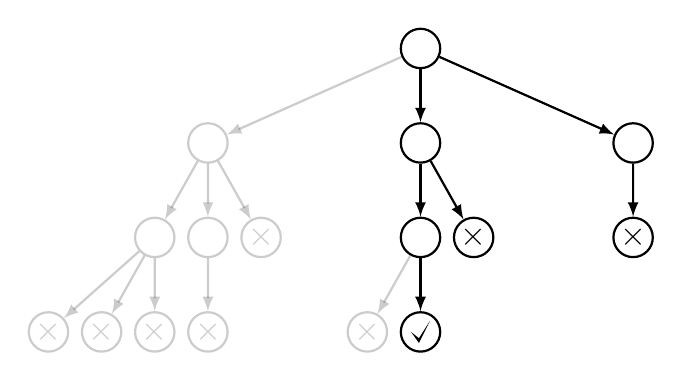
\begin{tikzpicture}[scale=.75, x=9mm, y=8mm]
			\def\checkmark{\tikz\fill[x=4mm, y=4mm](0, .35) -- (.25, 0) -- (.6, .7) -- (.25, .15) -- cycle;} 
			\tikzstyle{node}=[draw, thick, circle, inner sep=0pt, minimum width=5mm]
			\tikzstyle{node_}=[draw, thick, circle, inner sep=0pt, minimum width=5mm, opacity=.2]
			\large
			\node[node] (a) at (0, 6) {};
			\node[node_] (b1) at (-4, 4) {};
			\node[node] (b2) at (0, 4) {};
			\node[node] (b3) at (4, 4) {};
			\node[node_] (c11) at (-5, 2) {};
			\node[node_] (c12) at (-4, 2) {};
			\node[node_] (c13) at (-3, 2) {$\times$};
			\node[node] (c22) at (0, 2) {};
			\node[node] (c23) at (1, 2) {$\times$};
			\node[node] (c33) at (4, 2) {$\times$};
			\node[node_] (d111) at (-7, 0) {$\times$};
			\node[node_] (d112) at (-6, 0) {$\times$};
			\node[node_] (d113) at (-5, 0) {$\times$};
			\node[node_] (d122) at (-4, 0) {$\times$};
			\node[node_] (d221) at (-1, 0) {$\times$};
			\node[node] (d222) at (0, 0) {\checkmark};
			\draw[-{latex}, thick, opacity=.2] (a) edge (b1)  
			                 (b1) edge (c11) (b1) edge (c12) (b1) edge (c13)
			                 (c11) edge (d111) (c11) edge (d112) (c11) edge (d113)
			                 (c12) edge (d122)
			                 (c22) edge (d221);
			\draw[-{latex}, thick]
			                 (a) edge (b2)
			                 (a) edge (b3)
			                 (b2) edge (c22)
			                 (b2) edge (c23)
			                 (b3) edge (c33)
			                 (c22) edge (d222);
		\end{tikzpicture}
		\caption{Betrachteter Teilbaum von rechts nach links}
	\end{figure}
\end{minipage}